\documentclass{IEEEtran}
%% PACKAGES %%

\usepackage{amsmath, amsfonts, amssymb, amsthm}
\usepackage{braket}
\usepackage{listings}
\usepackage{geometry}
\usepackage{xcolor}
\usepackage{textcomp}
\usepackage{graphicx}
\usepackage{fancyhdr}
\usepackage{sourcecodepro}
\usepackage{multirow}

%%%%%%%%%%%%%%

\graphicspath{{./images}}

%% LISTINGS CONFIG %%

\definecolor{purple2}{RGB}{153,0,153} % there's actually no standard purple
\definecolor{green2}{RGB}{0,153,0} % a darker green

\lstset{
  basicstyle=\small\ttfamily,   % size of the fonts for the code
  frame = single,
  keywordstyle=\color{orange},       % core keywords
  keywordstyle={[2]\color{purple2}}, % built-ins
  stringstyle=\color{green2},%
  showstringspaces=false,
  commentstyle=\color{red},%
  upquote=true,                      % requires textcomp
  breaklines=true,
}

% Title Stuff
\title{ECE296 Lab 7 - Arduino Color Detector}
\author{Chase A. Lotito, \textit{SIUC Undergraduate}}
\date{}

\begin{document}

\maketitle % Makes the title

\section{Introduction} 
% (Brief description of how the lab was setup and the steps you took while completing the tasks given)

This experiment is the next step after the night light lab. Now, we replace the monochromatic LED with a RGB LED (Red-Green-Blue). The RGB LED will flash its colors against an object with a color that we wish to detect, and the photoresistor will see how much red, green, and blue the object reflects. Based on the intensities of reflection, we can set ranges for various colors--which let us tune the color detector accordingly.

\section{Assessment of Design}
% (How did it work in the end? Any problems or missteps along the way? Explain key aspects of design. Attach images of working design.)

Figure \ref{fig:design} shows the physical implementation of the color detector. 

\begin{figure}[!ht] 
    \centering
    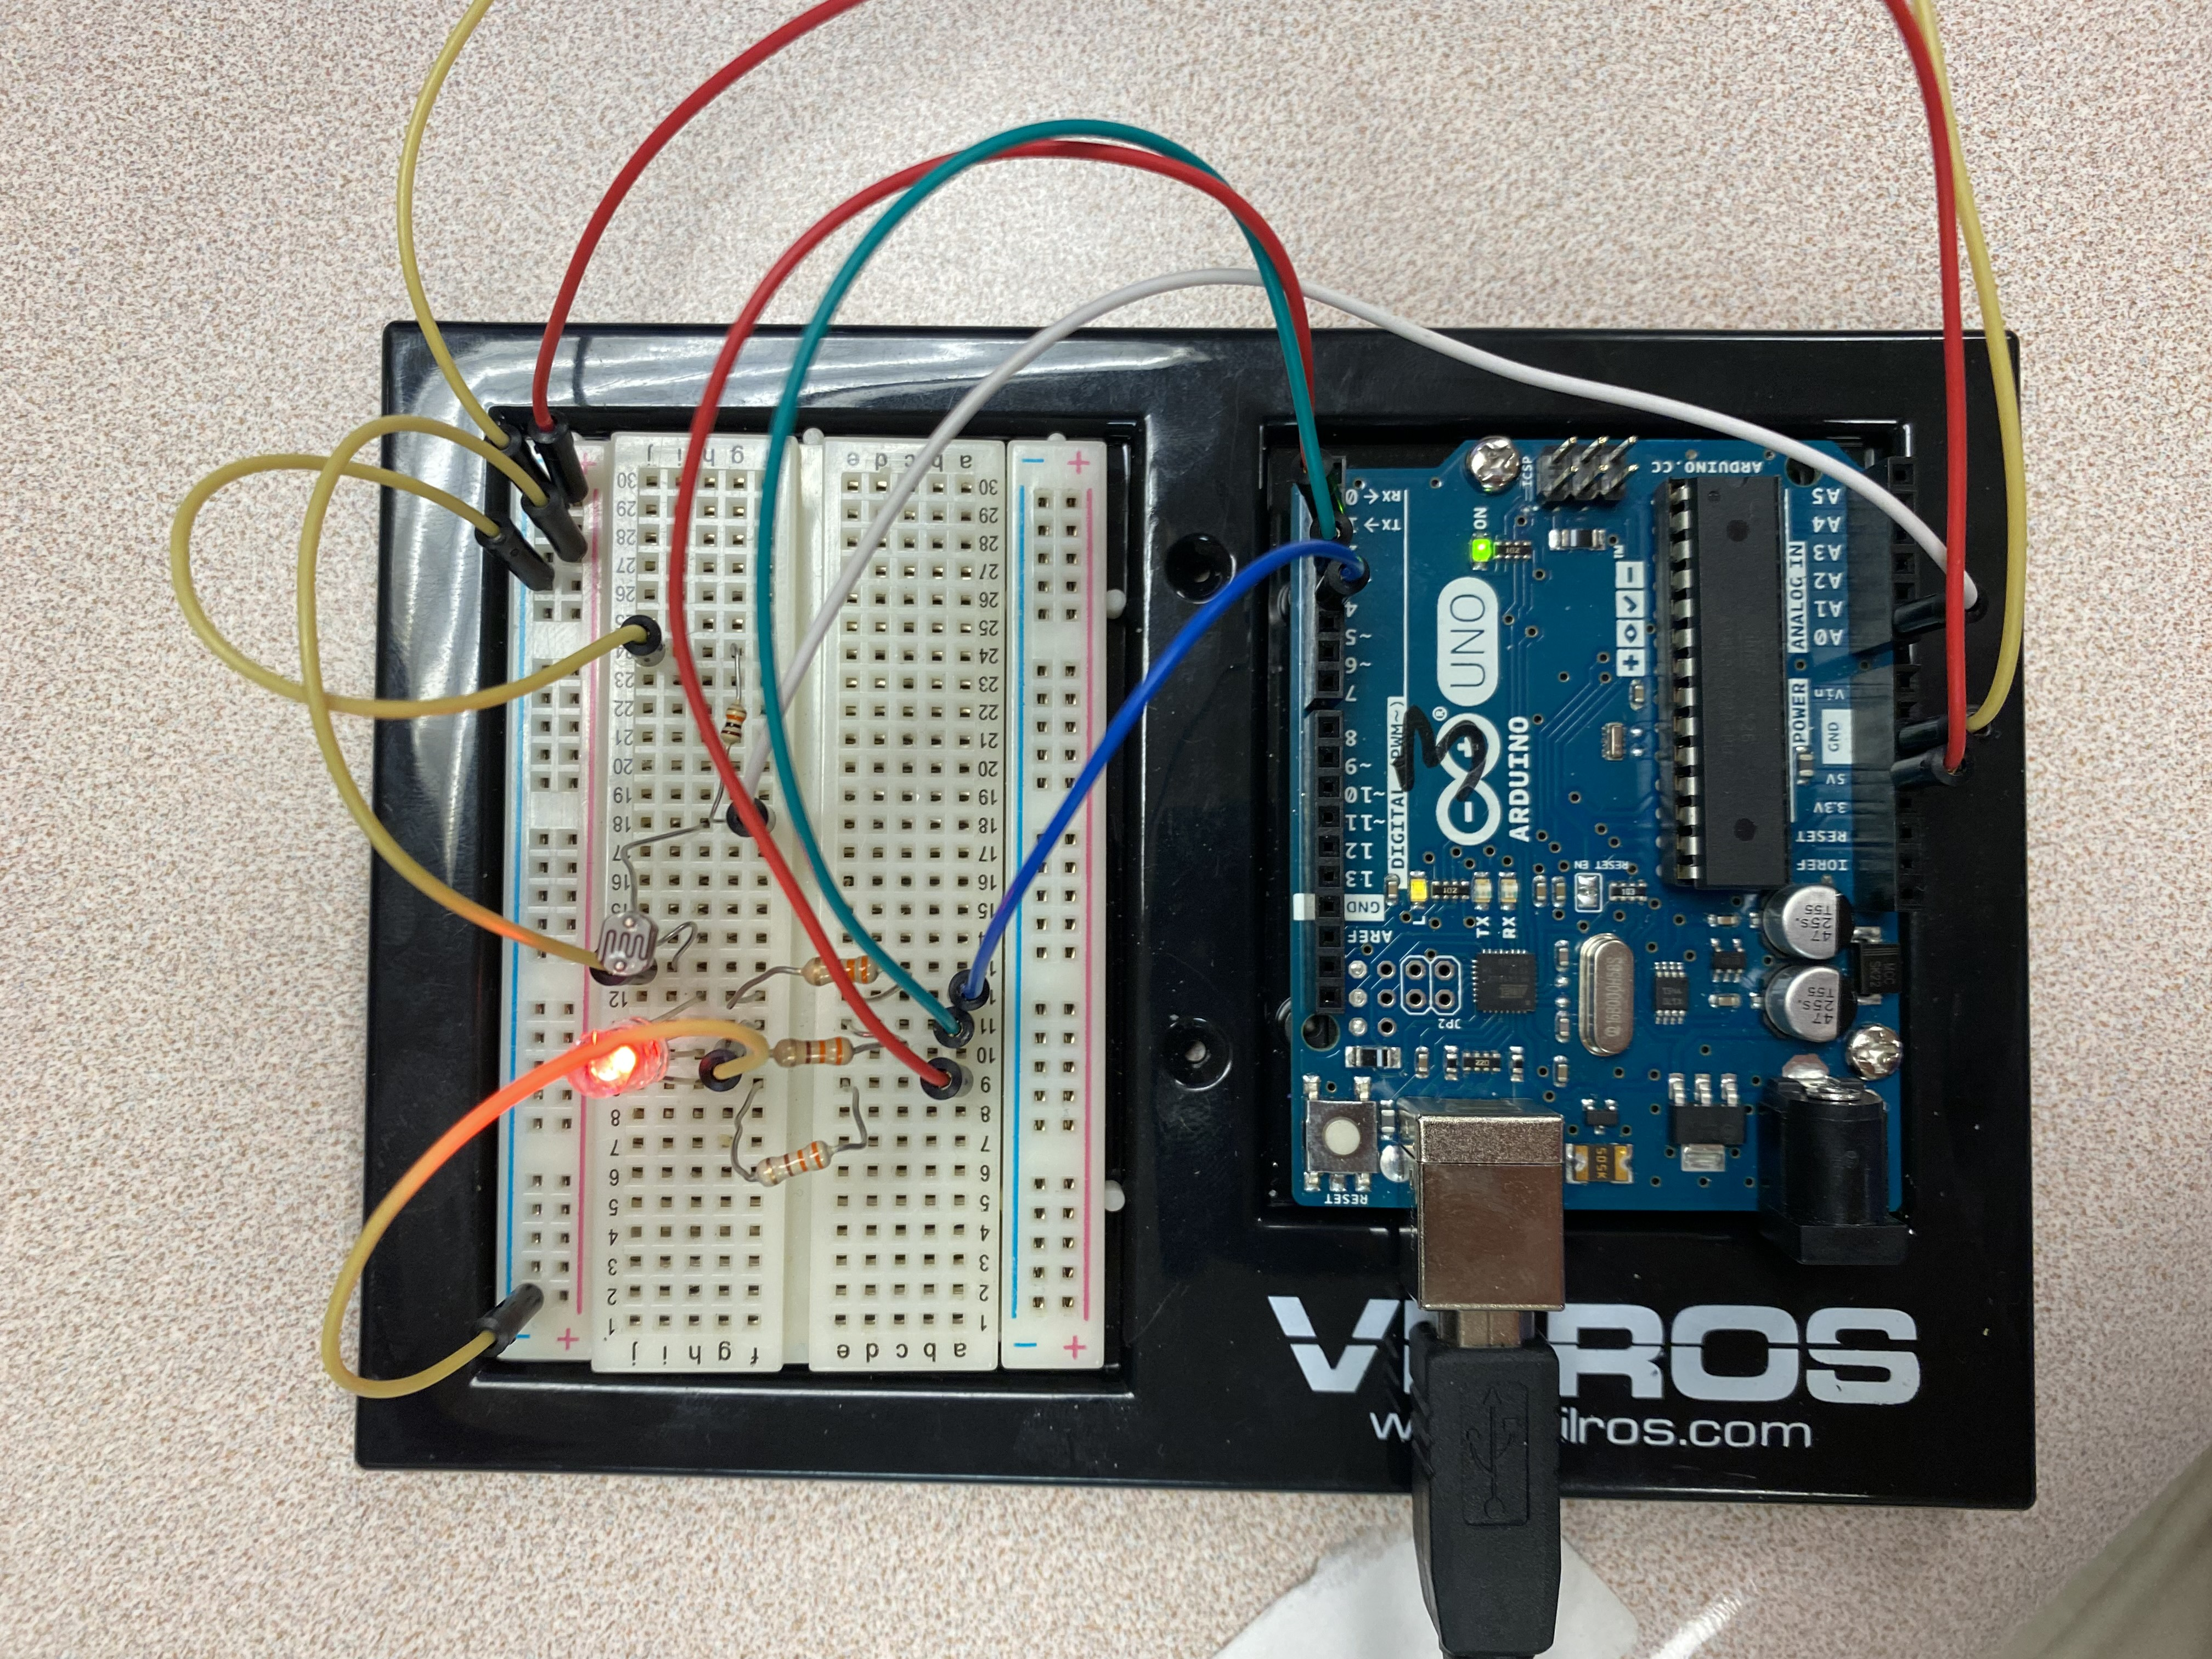
\includegraphics[width = 6cm]{color-detector-physical.jpeg}
    \caption{Color Detector Design}
    \label{fig:design}
\end{figure}

The circuit itself was difficult to tune; the sample colors were shown off of a phone screen, which caused volatility in brightness. However, the circuit was able to detect all 12 colors. 

The Arduino code flashes the LED red, then green, then blue, repeatedly in 100ms increments. Each individual pulse, we read the voltage between the photoresistor and \(10k\Omega\)-resistor, which via voltage-division should be between 0 and 5V. The \textit{analogRead()} function will translate this as an integer value between 0 and 1023. 

I personally kept this range intact, instead of using \textit{map()}, and this gave me a larger range to work with. The RGB values between successive colors tended to be small, so having a large range allowed more room for tolerances.

Finally, we collect the current RGB values detected from the photoresistor and send them through the \textit{if-else} conditional logic to find the correct color. The ranges for these can be referenced in the code in \textit{Appendix B}. The color detection is displayed on the Serial Monitor, and those can be seen in Figure \ref{fig:colorsDetected}.

\begin{figure}[!ht] 
    \centering
    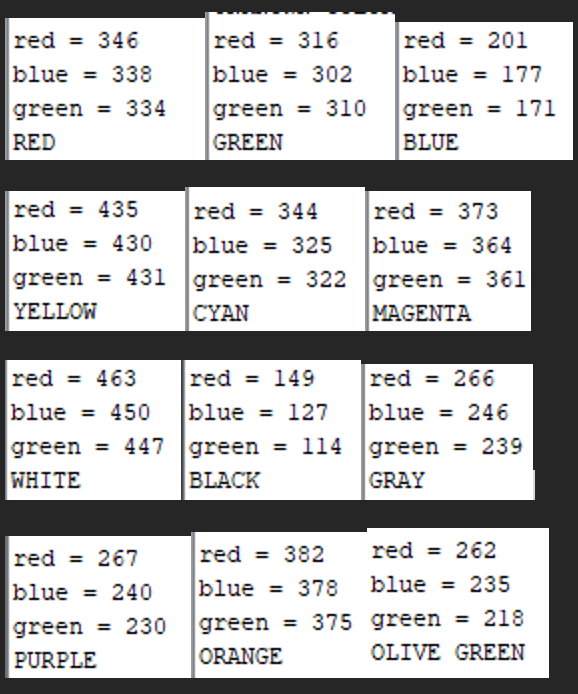
\includegraphics[width = 6cm]{colors-detected.png}
    \caption{All colors detected by circuit}
    \label{fig:colorsDetected}
\end{figure}

\section{Conclusion}
% (What did you learn during this lab? Final thoughts or findings? Did you meet the objectives? Answer any questions given in the lab manual here.)

Overall, this lab displayed the power of using solid-state devices with the Arduino to create useful sensors. Color detection seems like an extremely difficult task that would require AI image models, but all you need are simple passive components.

\section*{Appendix A: Hardware Schematic}

\begin{figure}[!ht] 
    \centering
    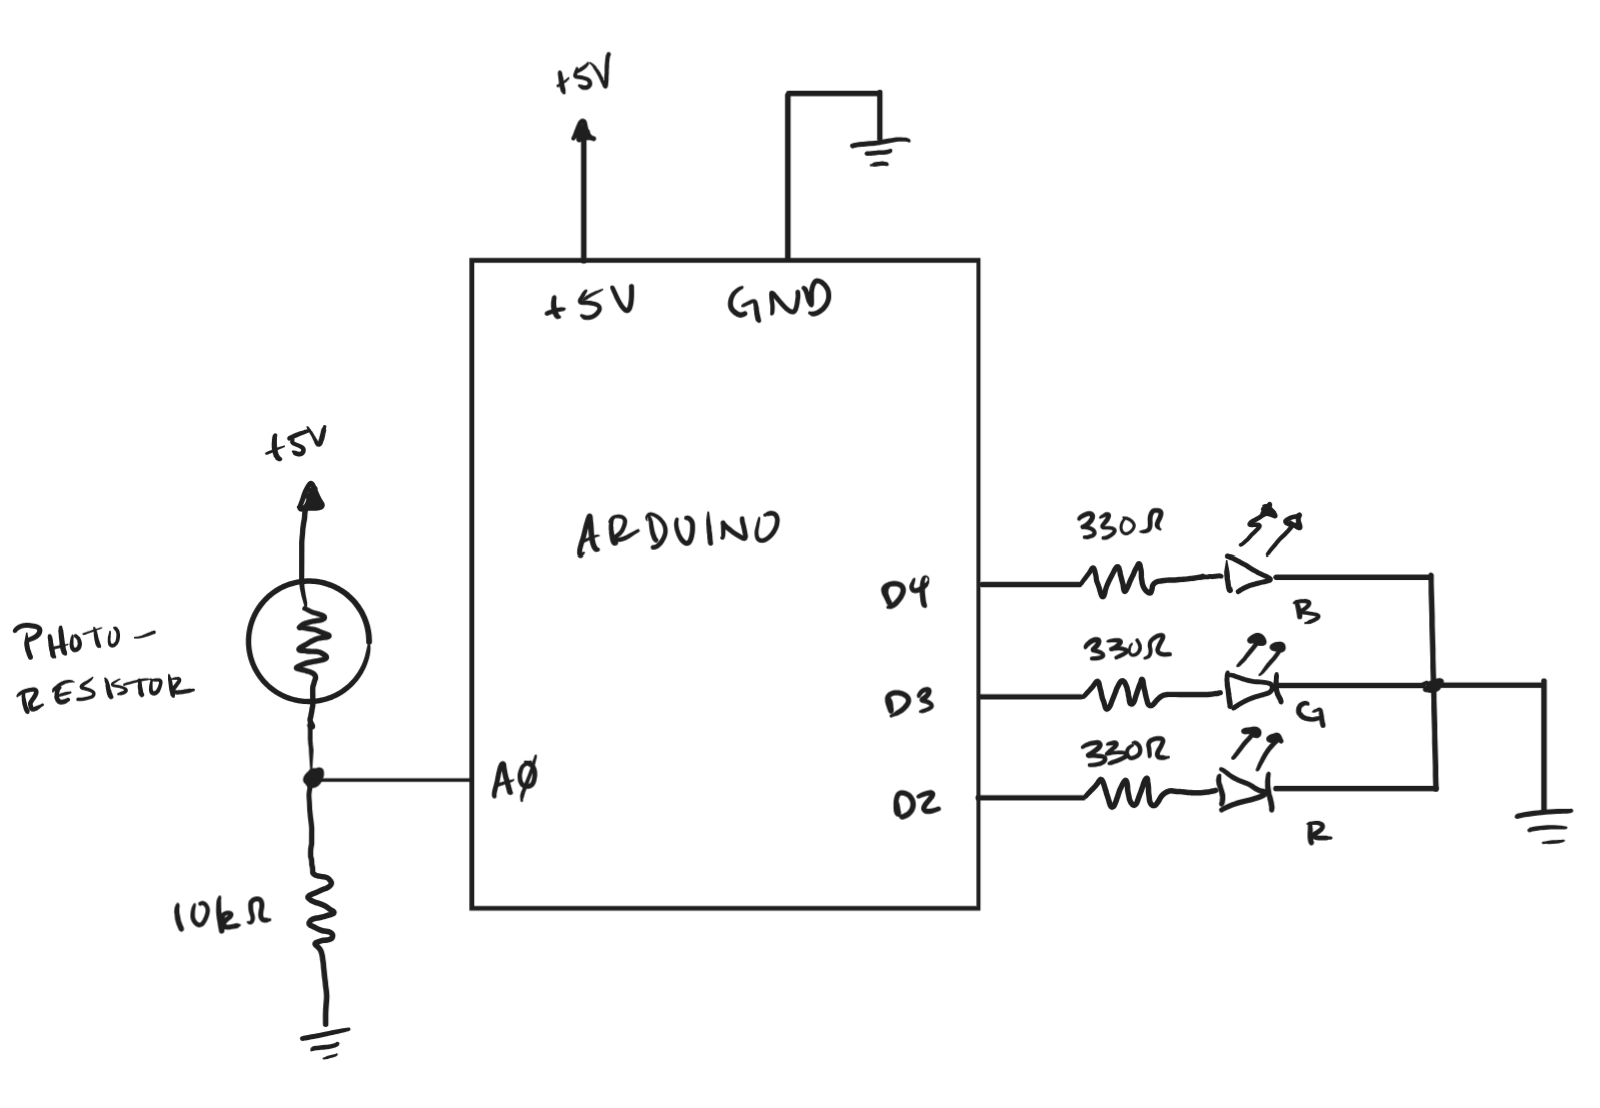
\includegraphics[width = 7cm]{color-circuit-diagram.png}
    \caption{Color Detector circuit diagram}
    \label{fig:colorCircuit}
\end{figure}

\section*{Appendix B: Code for the Software Developed}

\begin{lstlisting}
int red, blue, green;
int delay_time = 100;
int sensor;

void setup() {
    pinMode(2, OUTPUT); // Red
    pinMode(3, OUTPUT); // Blue
    pinMode(4, OUTPUT); // Green
    Serial.begin(9600);
}

void loop() {
    digitalWrite(2,HIGH);
    digitalWrite(3,LOW);
    digitalWrite(4,LOW);
    delay(delay_time);
    red = analogRead(A0);
    red = map(red, 230, 670, 0, 255);

    digitalWrite(2,LOW);
    digitalWrite(3,HIGH);
    digitalWrite(4,LOW);
    delay(delay_time);
    blue = analogRead(A0);
    blue = map(blue, 340, 675, 0, 255);

    digitalWrite(2,LOW);
    digitalWrite(3,LOW);
    digitalWrite(4,HIGH);
    delay(delay_time);
    green = analogRead(A0);
    green = map(green, 240, 666, 0, 255);

    Serial.print("red = ");
    Serial.println(red);
    Serial.print("blue = ");
    Serial.println(blue);
    Serial.print("green = ");
    Serial.println(green);

    if (red > 175 && blue < 176 && green > 168){
        Serial.println("RED");
    }
    else if (red < 183 && blue > 170 && green < 180){
        Serial.println("GREEN");
    }
    else if (red > 180 && blue > 205 && green < 182){
        Serial.println("CYAN");
    }
    else if (red < 200 && blue < 186 && green > 182){
        Serial.println("MAGENTA");
    }
    else if (red < 85 && blue < 85 && green > 35){
        Serial.println("BLUE");
    }
    else if (red < 245 && blue < 240 && green > 229) {
        Serial.println("YELLOW");
    }
    else if (red < 30 && blue < 2 && green < 0) {
        Serial.println("BLACK");
    }
    else if (red > 240 && blue > 240 && green < 255) {
        Serial.println("WHITE");
    }
    else {
        Serial.println("UNKNOWN COLOR");
    }
}
\end{lstlisting}

\end{document}
